\subsection{Glyph: \glyph{State variable}}
\label{sec:stateVariable}

Many biological entities such as molecules can exist in different states, meaning different physical or informational configurations.
These states can arise for a variety of reasons.
For example, macromolecules can be subject to post-synthesis modifications, wherein residues of the macromolecules (amino acids, nucleosides, or glucid residues) are modified through covalent linkage to other chemicals.
Other examples of states are alternative conformations as in the closed/open/desensitised conformations of a transmembrane channel, and the active/inactive forms of an enzyme.

To describe such states, the \PD introduces the concept of the state variable.
A state variable of a biological entity usually has a name (\eg ``S122'' to indicate residue Serine 122 of a protein), and can be assigned a value (\eg ``P'', to indicate a phosphate group).
Such a state variable models a dimension along which the state of the overall entity can vary.
The state of an entity can then be described by the current values assigned to all its state variables, and of all its possible components, recursively.
A state variable may be assigned no value; an example of a situation where this might arise is an unphosphorylated phosphorylation site.
A state variable might also be unnamed, in cases where there is no ambiguity between this state variable and another state variable carried by the same entity (\eg when an entity carries a unique state variable, it might be unnamed).
In \PD, state variables, together with the values assigned to them, are represented using the \glyph{state variable} glyph.

\begin{glyphDescription}

\glyphSboTerm
Not applicable.

\glyphIncoming
None.

\glyphOutgoing
None.

\glyphContainer
A \glyph{state variable} is represented by a ``stadium'' shape, that is two semicircles of the same radius joined by parallel segments, as shown in \novreffig{state-var}.

The centre of the shape should be placed on the border of the EPN.

In previous versions of this specification, the \glyph{state variable} was represented by an elliptic shape.
This symbol is now \textbf{deprecated} in favour of the stadium shape described above.

\glyphLabel
A \glyph{state variable} is identified by a label that is a string of characters.
The characters cannot be distributed on several lines.
The centre of the label must be placed on the centre of the container.
The label may extend outside of the container.
The label is constituted of two substrings separated by the character ``@'', the first one indentifying the value of the state variable, and the second one its name.
The character ``@'' is omitted when the state variable is unnamed.
In previous versions of this specification, the substring identifying the name of the state variable was allowed to be displayed using a second label, placed outside of the shape. This alternative approach is now deprecated with this version.

\glyphAux
None.

\end{glyphDescription}

\begin{figure}[H]
  \centering
  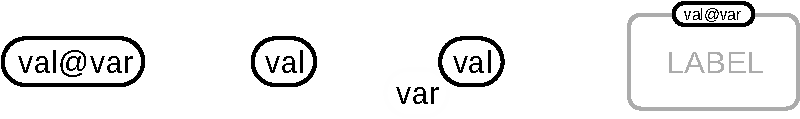
\includegraphics{images/build/state_variable.pdf}
  \caption{The \PD glyph for \glyph{state variable}, shown with a value and a variable on the far left, with only a value on the middle-left, with an additional label for the variable on the middle-right (deprecated), and decorating a \glyph{macromolecule} (\sect{macromolecule}) on the far right.}
  \label{fig:state-var}
\end{figure}

\begin{figure}[H]
  \centering
    \begin{tabular}{lc}
        A & \raisebox{-\height}{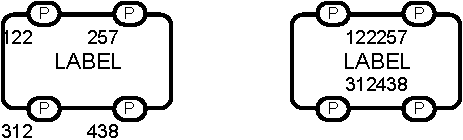
\includegraphics{images/build/wrong_state_variables_a_example.pdf}}\\
        B & \raisebox{-\height}{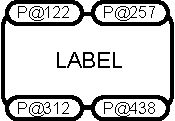
\includegraphics{images/build/wrong_state_variables_b_example.pdf}}
    \end{tabular}
  \caption{A. Examples of discouraged use of \glyph{state variables}. B. Encouraged use.}
 \label{fig:wrong-state-var}
\end{figure}
